\chapter{Reductions: Importing Hardness into Database Problems}
\label{ch:reduction}

Most ``impossible'' statements in database research are not proved from scratch: they are
\emph{imported}. A reduction exhibits a computable translation from a problem already
believed hard --- CLIQUE, Set Cover, inner-product estimation, hyperclique detection ---
into the problem at hand, so that any algorithm, approximation, private mechanism, or
sampler for the target would also solve the source. Reductions are the most used
theoretical tool in our SIGMOD'26 corpus: 50 of 228 tagged papers rely on them, and 32 of
those pair a reduction with an explicit hardness claim. They matter in both directions:
they delimit what any system can do (lower bounds, dichotomies, inapproximability) and,
run backwards, they turn new problems into old ones with known algorithms.

\section{The tool: mappings that preserve what you care about}

\begin{definition}[Polynomial-time many-one reduction]
Let $L_1, L_2$ be decision problems. We write $L_1 \le_m^p L_2$ if there is a
polynomial-time computable function $f$ with $x \in L_1 \iff f(x) \in L_2$ for all $x$.
If some NP-hard $L_1$ reduces to $L_2$, then $L_2$ is NP-hard: a polynomial-time
algorithm for $L_2$, composed with $f$, would decide $L_1$.
\end{definition}

This is the classical core \cite{reduction-bg2,reduction-bg1,reduction-bg3}, and it
already reaches into databases.

\begin{example}[Conjunctive-query evaluation is NP-complete]
Given $(G,k)$, build in polynomial time the database $D_G$ holding the edge relation of
$G$, and let $Q_k$ be the conjunctive query
\[
Q_k \;=\; \exists v_1 \dots \exists v_k \,.\, \bigwedge_{1 \le i < j \le k} E(v_i, v_j).
\]
Then $G$ has a $k$-clique iff $Q_k(D_G) \ne \emptyset$. Since CLIQUE is NP-complete, CQ
evaluation is NP-hard (and it lies in NP) --- the starting point of query-evaluation
complexity \cite{reduction-bg6}.
\end{example}

Decision-hardness is often not enough: DB problems carry objectives (cost, error,
latency), so the reduction must preserve \emph{quality}, not just yes/no membership.

\begin{definition}[$L$-reduction, i.e., approximation-preserving reduction]
Optimization problem $A$ L-reduces to $B$ if there are polynomial-time maps $f$
(instances) and $g$ (solutions) and constants $\alpha, \beta > 0$ such that, for every
instance $x$ of $A$, writing $c_A, c_B$ for the objective values:
(i)~$\mathrm{OPT}_B(f(x)) \le \alpha \cdot \mathrm{OPT}_A(x)$; and
(ii)~every solution $y$ of $f(x)$ maps to a solution $g(y)$ of $x$ with
$|c_A(g(y)) - \mathrm{OPT}_A(x)| \le \beta \cdot |c_B(y) - \mathrm{OPT}_B(f(x))|$.
\end{definition}

\begin{proposition}
If $A$ L-reduces to $B$ with constants $\alpha,\beta$ and $B$ admits a polynomial-time
$r$-approximation, then $A$ admits an $\alpha\beta r$-approximation. Hence hardness of
\emph{approximating} $A$ --- e.g., Set Cover's $\log n$ threshold under the Unique Games
Conjecture --- transfers to $B$ \cite{reduction-bg4,reduction-bg1}.
\end{proposition}

\begin{remark}[Fine-grained and conditional reductions]
When polynomial versus exponential time is too coarse, the source problem $H$ carries a
quantitative hypothesis (SETH, combinatorial Boolean matrix multiplication, hyperclique
detection, listing lower bounds) \cite{reduction-bg5}. The reduction must then track
parameters: an algorithm for $P$ with cost $c_P$ on instances produced by $f$ yields an
algorithm for $H$ of cost (cost of $f$) $+$ (number of calls) $\cdot\, c_P$, and the
hypothesis transfers whenever this beats the assumed lower bound in every parameter
regime.
\end{remark}

The same skeleton covers quantitative guarantees: replace ``algorithm'' by ``mechanism
or estimator with error $\alpha$,'' and the reduction lifts accuracy instead of time.
Figure~\ref{fig:reduction-skeleton} schematizes the two halves.

\begin{figure}[t]
\centering
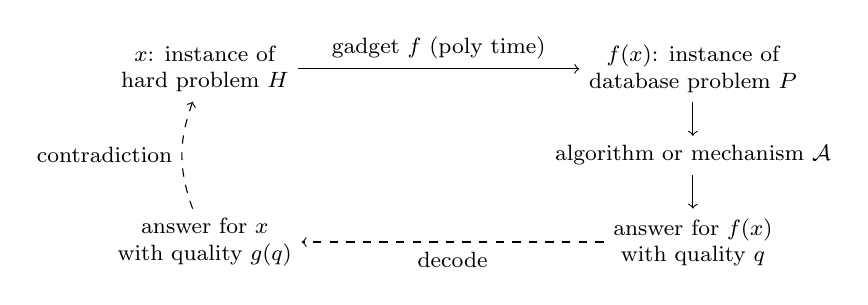
\begin{tikzpicture}[every node/.style={font=\footnotesize, align=center}]
  \node (xl) at (0,1.1) {$x$: instance of\\ hard problem $H$};
  \node (fl) at (6.2,1.1) {$f(x)$: instance of\\ database problem $P$};
  \node (al) at (6.2,0) {algorithm or mechanism $\mathcal{A}$};
  \node (dl) at (6.2,-1.1) {answer for $f(x)$\\ with quality $q$};
  \node (bl) at (0,-1.1) {answer for $x$\\ with quality $g(q)$};
  \draw[->] (xl) -- node[above] {gadget $f$ (poly time)} (fl);
  \draw[->] (fl) -- (al);
  \draw[->] (al) -- (dl);
  \draw[->,dashed] (dl) -- node[below] {decode} (bl);
  \draw[->,dashed] (bl) to[bend left=20] node[left] {contradiction} (xl);
\end{tikzpicture}
\caption{Every reduction has two halves: instances travel forward through the gadget;
solutions --- or accuracy, or privacy --- travel backward, so quality achieved for $P$
becomes quality for $H$.}
\label{fig:reduction-skeleton}
\end{figure}

\section{Reductions at work in the SIGMOD'26 corpus}

\subsection{Gadget reductions: privacy under continual release}

A stream of edge updates arrives over $T$ timesteps, and an $(\varepsilon,
\delta)$-differentially private mechanism must continually report, on $n$-node graphs,
the size of the maximum matching, the degree histogram, or the core number of a vertex.

\begin{theorem}[Continual-release lower bound]
Let $\varepsilon \in [0,1]$ and $\delta \in [0,1/3]$. Any $(\varepsilon, \delta)$-DP
incremental mechanism in the exact setting for maintaining the size of the maximum
matching, the degree histogram, or the core number of a vertex must have additive error
$\alpha = \Omega\bigl(\min\{ T^{a},\, n^{b} \}\bigr)$, for problem-specific constants
$a, b \in [1/8, 1/2]$.
\end{theorem}

The reduction embeds an \textsc{InnerProduct} instance of dimension $d$ into the update
stream via \emph{extendable bitwise-AND gadgets} with $v(d)$ vertices and $t(d)$ edges
(for matching, $v(d) = t(d) = O(d^2)$): a mechanism with additive error $\alpha$ would
answer the inner product within $2\alpha$, forcing
$\alpha = \Omega(\min\{ t^{-}(T), v^{-}(n) \})$ for generalized inverses, with $d$ chosen
exactly as that minimum. Binary-tree mechanisms with DP composition give near-matching
upper bounds, so the reduction is essentially tight. \cite{sigmod26-136}\pods

\subsection{Gap reductions: clustering with set outliers}

Points are clustered while whole \emph{sets} may be discarded as outliers: given points
$P$, a family $\mathcal{H}$ of candidate outlier sets (hyper-rectangles, or sets induced
by a relational join), and budgets $k, z$, choose at most $k$ centers and at most $z$
outlier sets so as to minimize the cost of the uncovered points.

\begin{theorem}[Inapproximability under the Unique Games Conjecture]
If the Unique Games Conjecture is true, there exists no $(1, f - \varepsilon,
\gamma)$-approximation algorithm that runs in polynomial time for the problem, whenever
$f = o(\log n)$, where the triple bounds the clustering-cost factor and the allowed
violation of the center and outlier budgets.
\end{theorem}

The reduction is a line--point encoding of Set Cover: element $x_i$ becomes the point
$p_i$ at coordinate $i$, each set $y$ becomes the outlier set $\{ p_i : x_i \in y \}$,
and singleton sets pad the family, so covering the element-points with at most $z$
outlier sets is exactly a set cover --- and Set Cover's UGC-conditional $\log n$
threshold crosses over. The same paper runs the machinery constructively: LP feasibility
with greedy rounding, weight-charging, and coresets yield $(2 + \varepsilon, 2,
O(1))$-approximations, including over acyclic joins. \cite{sigmod26-289}

\subsection{Coupon-collector reductions: sampling join--project queries}

For a join--project query $Q$ (a join followed by projection, so duplicates disappear),
with input size $N$ and output size $\mathsf{OUT}$, the paper asks what uniform sampling
from, and approximate counting of, $Q(I)$ must cost after indexing.

\begin{theorem}[Conditional bound for star queries]
For the star query $Q_k$, assuming the combinatorial hardness of listing star-join
results (any combinatorial listing algorithm requires
$\Omega(N \cdot \mathsf{OUT}^{1-1/k})$ time, under the property-testing model), no
combinatorial algorithm can preprocess an instance of input size $N$ and output size
$\mathsf{OUT}$ in $O(N \cdot \mathsf{OUT}^{1/k-\gamma})$ time and then return a uniform
sample from $Q(I)$ in $O(\mathsf{OUT}^{1/k+\gamma})$ expected time, for any constant
$\gamma > 0$.
\end{theorem}

The reduction runs the coupon collector backwards: a sampler this fast would list all
$\mathsf{OUT}$ results after $\mathsf{OUT} \log \mathsf{OUT}$ draws and thereby beat the
assumed listing lower bound. For the matrix query the hypothesis is instantiated by the
combinatorial hardness of Boolean matrix multiplication (the case $k=2$), and any
randomized algorithm that outputs an $O(1)$-approximation of $\mathsf{OUT}$ with high
probability requires at least $\Omega(N / \sqrt{\mathsf{OUT}})$ time; heavy/light
partitioning with Hoeffding intersection estimation gives matching upper bounds.
\cite{sigmod26-243}\pods

\subsection{Fine-grained reductions: direct access with min/max aggregates}

In direct access, the database is preprocessed once so that answers to an acyclic
free-connex conjunctive query can be enumerated in a user-chosen order with constant
delay; the question is which aggregate-driven orders, such as sorting by $\min X$, admit
quasilinear-time preprocessing.

\begin{theorem}[Hard side of the dichotomy]
Direct access according to $\min X$ is not possible in quasilinear time if $Q$ has a
chordless $k$-path ($k \ge 3$) between two variables in $X$, assuming the Hyperclique
hypothesis and SETH.
\end{theorem}

The reduction encodes triangle and hyperclique detection so that a quasilinear-time
direct-access structure for $\min X$ would decide hyperclique existence faster than the
hypothesis permits. The easy side of the dichotomy is algorithmic: strict total orders
are partitioned into partial orders that suitably rearranged join trees enforce, after
existential variables are eliminated in linear time. \cite{sigmod26-109}\pods

\begin{reachbox}{When to reach for reductions}
\begin{itemize}
\item \textbf{Lower bounds without a from-scratch proof.} Pick the canonical hard
problem closest in shape (Set Cover for covering and outlier budgets, InnerProduct for
private estimation, hyperclique detection for join patterns, listing for enumeration),
build a gadget, and state explicitly which hypothesis the reader inherits.
\item \textbf{Hardness of approximating, not just deciding.} Make the reduction
gap-preserving (an $L$-reduction), so the source's inapproximability threshold --- not
merely its NP-hardness --- crosses over to your objective.
\item \textbf{Fine-grained statements.} When the target is a refined running time
(sublinear, output-sensitive, constant delay), condition on a quantitative hypothesis
and audit the parameter blow-up of the gadget; a sloppy parameter map makes the bound
vacuous in some regime.
\item \textbf{Reductions also certify tractability.} The same machinery run backwards
--- encoding your problem into LP feasibility, matchings, or coresets --- builds the
upper-bound side of a dichotomy.
\end{itemize}
\end{reachbox}
